\documentclass{article}
\usepackage[utf8]{inputenc}
\usepackage{lipsum}
\usepackage{authblk}
\usepackage{chngpage}
\usepackage{pdflscape}
\usepackage{amsfonts}
\usepackage{paralist}

\usepackage[
  textwidth=18mm,
  textsize=tiny,
  linecolor=orange,
  colorinlistoftodos]{todonotes}

\title{Research and Implementation of Deterministic Graph Exploration with Advice: Final report}
\author[1]{Dorottya Benyovszki}
\author[1]{Anna Böndicz Georgina}
\author[1]{Kristóf Umann}
\affil[1]{Eötvös Loránd University, Faculty of Informatics}
\date{\today}

%\input{preamble_tikz.tex}
%\input{preamble_lstlisting.tex}

\begin{document}

\maketitle

\begin{abstract}
  Consider an $n$-node undirected graph, where each node $u$ with degree $d$ arbirarily assigns port numbers $0,\dots,d-1$ to each of its edges. Now, consider a robot starting in an arbitrary position in this graph; in each node, the robot can learn about which edged it can traverse through by reading the available port numbers, can keep track of the ports taken, and may track the port numbers to return to its starting position. However, in the absence of node labels, the robot can never be sure of its position in the graph, and requires some outside help to visit every node in it. For this reason, an outsider entity, knowledgable about the graph, called an \textit{oracle} provides an advice to the robot before it starts exploring. The quality of the advice, bound by its length in bits, affects the exploration time (the amount of nodes visited before visiting each at least once) of the robot.

  In this final report, we discuss the implementation and simulation results of the program inspired by \cite{gorain2018deterministic}. We focus on the case of a \textit{map oracle} giving advice to the robot, which is unaware of the starting position of the robot. Using the advice from a map oracle, the robot will construct routes for each node of the graph, and attempt to explore them one-by-one. We found that the robot will successfully greater number of these routes then expected. We show that the more edges a given graph has relative to its node count, the likelyhood of a given route leading to a successful exploration of the graph is greater.

\end{abstract}

\section{Introduction}
\label{sec:introduction}

The problem of exploring a graph with a robot in fact describes a diverse set of problems: the use of tethered robots that can travel only so far from their start, or robots that need to periodically refuel at certain nodes offer and interesting layer of difficulty. Nonetheless, we discuss a rather simple version of this problem. Consider a graph with $n$ nodes. Each node $u$ with degree $d$ arbirarily assigns label numbers $0,\dots,d-1$ to each of its edges. We call these edge labels (of which each edge has two) port numbers. The lack of node labels and the arbitrarity of the labeling makis it such that any entity traversing this graph without prior knowledge of any of its properties is unable to tell which nodes has it already visited.

The robot, though we allow for infinite fuel and no tether, is still rather primitive. It has no prior knowledge of the graph on its own, in each node, it can learn about which edged it can traverse through by reading the available port numbers, can keep track of the ports taken, and may track the port numbers to return to its starting position. Figure \ref{fig:port-numbered-graph} demonstrated a robot being in a port numbered graph.

An outsider entity, knowledgable about the graph, called an \textit{oracle} provides an advice to the robot once, before it starts exploring. The quality of the advice affects the exploration time (the amount of nodes visited before visiting each at least once) of the robot. We discuss the quality in terms of size in bits. An \textit{instance oracle} also knows the starting position of the robot in the graph, while a \textit{map oracle} does not. As the more challenging case, we chose to focus on map oracles.

In a shorter advice, an oracle may only be able to provide limited information, like the number of nodes in the graph, or more severe yet, an upper bound of said number. Our implementation is more lenient, and allows the encoding of a spanning tree in the graph, resulting in an advice of size $\mathbb{O}(n)$. In the case of a map oracle, however, this still forces the robot to attempt, and occasionally fail to explore certain routes. The rate of success has become our primary focus during our research: we show that the denser a graph is (the more edges it has relative to the number of nodes), the morel likely is a route to successfully traverse the graph.

\begin{figure}
  \centering
  \includegraphics[width=\columnwidth]{figures/port_numbered_graph.png}
  \caption{A port numbered graph.}
  \label{fig:port-numbered-graph}
\end{figure}

\section{Our chosen algorithm}
\label{sec:algorithm}


\begin{figure}
  \textbf{Input:} Initial graph $G$

  \textbf{Output:} An advice in binary representation
  \vspace{1em}

  \begin{compactenum}
  \item Create a spanning tree $T$ in $G$, rooted at some arbitrary node.
  \item \label{prev}Encode $T$ in order of a DFS traversal such that
    \begin{compactenum}
    \item bit 1 means to ,,go down in the tree'' to a previously unexplored node,
    \item bit 0 means to ,,go up the tree''.
    \end{compactenum}
  \item Write as many 0s as is needed to ,,go back'' to the root of $T$. Write another 0, signaling the end of the bits describing the structure of $T$.
  \item Encode the port numbers as they are encountered following the euler route described in point \ref{prev}.
  \item Convert decimal port numbers to binary, pad them with 0s until the width reaches $\lceil\log_2(n)\rceil$.
  \end{compactenum}
  \caption{Advice construction for the map oracle.}
  \label{fig:encoding-alg}
\end{figure}


\begin{figure}
  \textbf{Input:} Advice constructed on Figure \ref{fig:encoding-alg}, initial graph $G$, and starting position $s$ (The robot itself is oblivious to the graph and its starting position in it.)

  \textbf{Output:} Port sequence that explores every node in the graph
  \vspace{1em}

  \begin{compactenum}
  \item Create the spanning tree $T$ with the appropriate port numbering.
  \item for each $u$ node in $T$,    
    \begin{compactenum}
      \item Identify an euler route in $T$ starting in $u$ and encode its port numbers in $E(u)$
      \item Let $E'(u)$ be the reverse of $E(u)$, and $F(u)$ the concatenation of $E(u)$ and $E'(u)$
      \item Attempt to traverse the graph following $F(u)$; if any port numbers does not exist, track back to the $s$
    \end{compactenum}
  \end{compactenum}
  \caption{Robot traversing the graph with an advice constructed on Figure \ref{fig:encoding-alg}.}
  \label{fig:ulgt-algorithm}
\end{figure}

\begin{figure}
  \centering
  \includegraphics[width=6cm]{figures/encoding.png}
  \caption{Encoding of a tree. Structure: 101011, 0s back to start and separator: 000, port numbers: 010 000 000 000 001 001 000 000}
  \label{fig:encoding}
\end{figure}

\section{Measurement methodology}
\label{sec:method}


\section{Results}
\label{sec:results}

\begin{landscape}
\begin{figure}
  \vspace{-2.9cm}
  \centering
  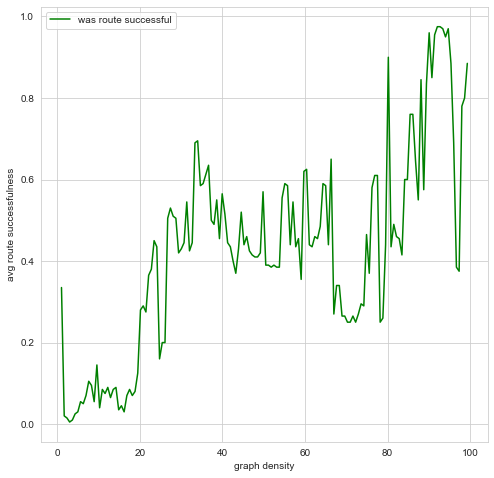
\includegraphics[width=8cm]{figures/random_uj/edge_den_succ.png}
  \hspace{1cm}
  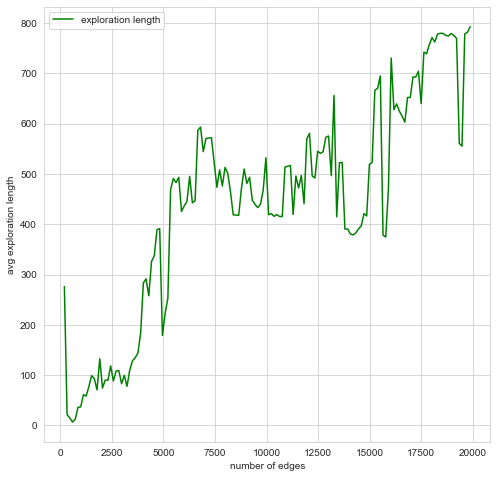
\includegraphics[width=8cm]{figures/random_uj/edge_expl.png}
  \vspace{1cm}

  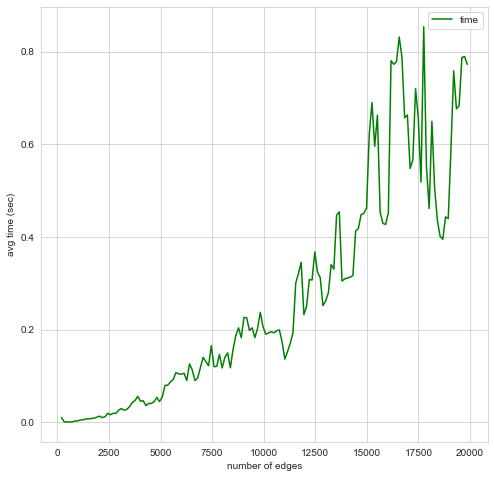
\includegraphics[width=8cm]{figures/random_uj/edge_time.png}
  \hspace{1cm}
  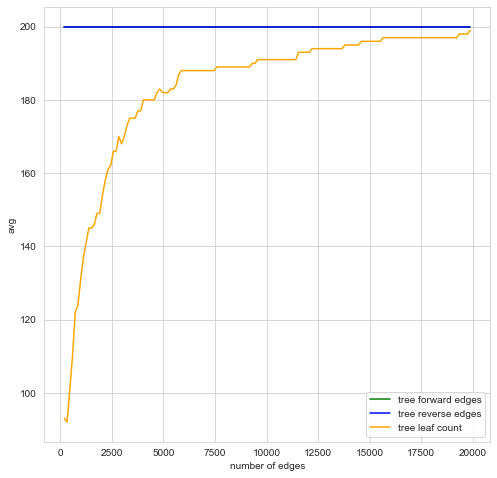
\includegraphics[width=8cm]{figures/random_uj/edge_tree.png}

  \caption{Measurements on increasing edge density. All graphs had 1000 nodes, and there were 10 additional and 10 excess edges.}
  \label{fig:edge-density}
\end{figure}
\end{landscape}

\begin{landscape}
\begin{figure}
  \vspace{-1.7cm}
  \centering
  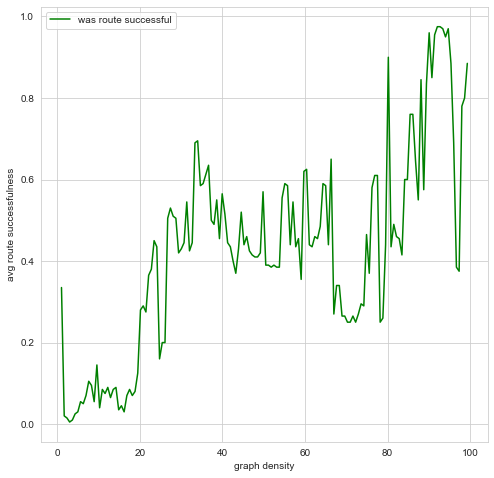
\includegraphics[width=0.48\columnwidth]{figures/random_uj/edge_den_succ.png}
  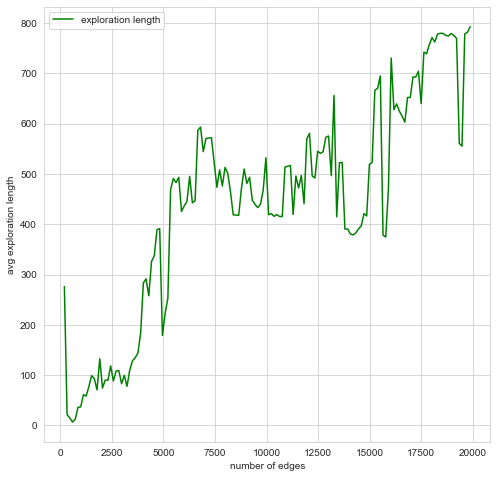
\includegraphics[width=0.48\columnwidth]{figures/random_uj/edge_expl.png}

  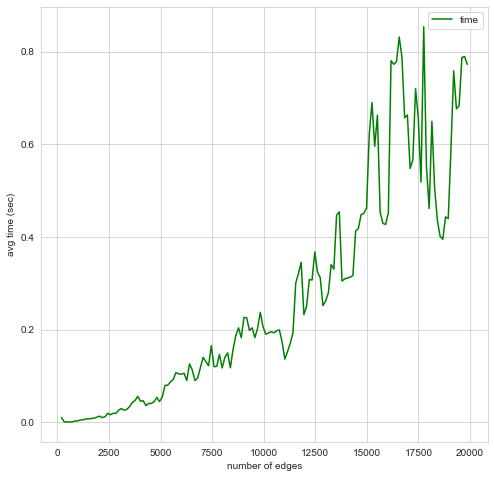
\includegraphics[width=0.48\columnwidth]{figures/random_uj/edge_time.png}
  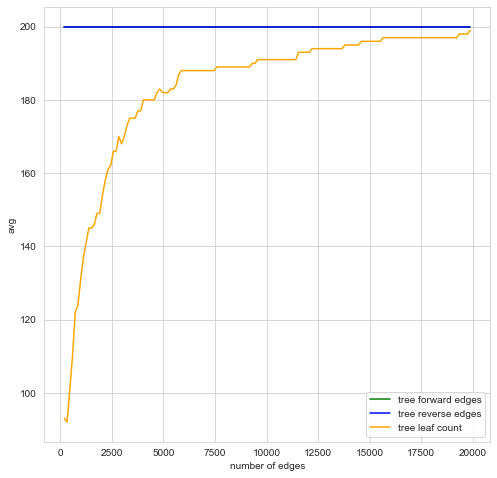
\includegraphics[width=0.48\columnwidth]{figures/random_uj/edge_tree.png}

  \caption{Measurements on increasing edge density. All graphs had 1000 nodes, and there were 10 additional and 10 excess edges.}
  \label{fig:edge-density}
\end{figure}
\end{landscape}

\begin{landscape}
\begin{figure}
  \vspace{-1.7cm}
  \centering
  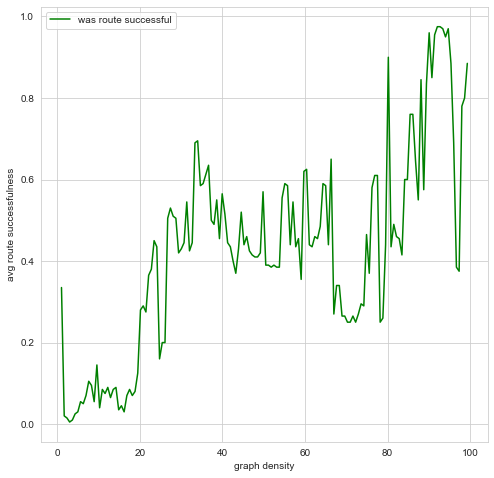
\includegraphics[width=0.48\columnwidth]{figures/random_uj/edge_den_succ.png}
  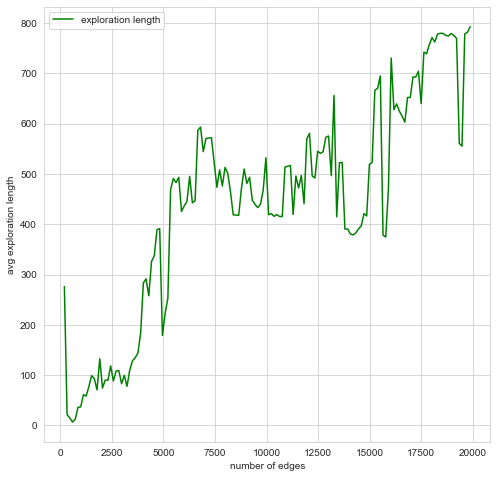
\includegraphics[width=0.48\columnwidth]{figures/random_uj/edge_expl.png}

  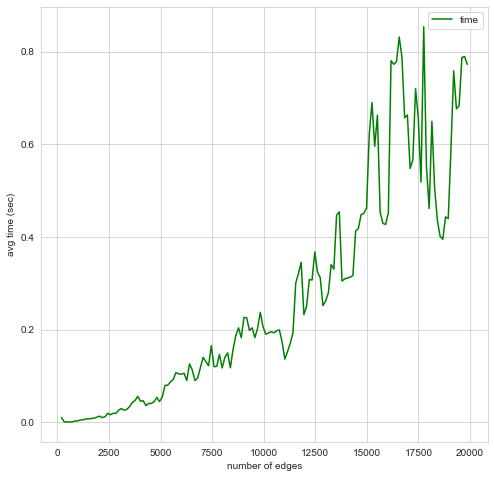
\includegraphics[width=0.48\columnwidth]{figures/random_uj/edge_time.png}
  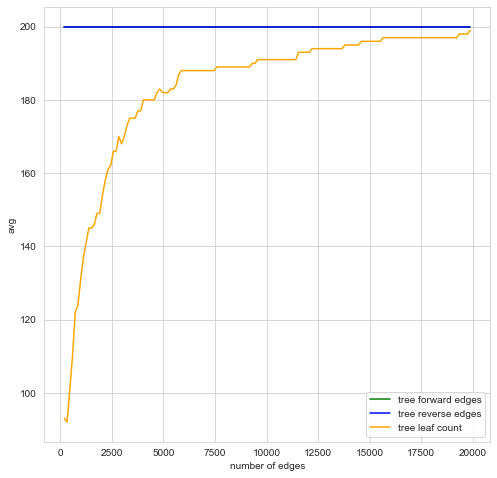
\includegraphics[width=0.48\columnwidth]{figures/random_uj/edge_tree.png}

  \caption{Measurements on increasing edge density. All graphs had 1000 nodes, and there were 10 additional and 10 excess edges.}
  \label{fig:edge-density}
\end{figure}
\end{landscape}

\section{Future work}
\label{sec:future-work}



\section{Conclusion}


\bibliographystyle{IEEEtran}
\bibliography{IEEEabrv,references}

\end{document}

